\chapter{List of transfer functions}
In our book, we mentioned a lot about specifically transfer functions in the neural construction. For convenience, here we summarize almost all transfer function of interest. What they are for? No idea (read the book, god-damn it!), but we will just search for them in here for a while, I guess. 

\section{Classical transfer functions}
A lot of transfer function, or rather the modern derivative of it in the classical sense, can be taken from \cite{10.5555/2721661}. Here, the transfer function can be linear or nonlinear function, in which it is used to transform the input-output characteristic of a single-input neuron into the variety of the transfer function. 
\subsection{Hard limit (\texttt{hardlim[x]})}
The hard limit transfer function, used in distinctive categorical sorting, has its input-output characteristic as: 
\begin{equation}
    \texttt{hardlim}[x] = \begin{cases}
        0 & x < 0\\
        1 & x \geq 0
    \end{cases}
\end{equation}
\begin{figure}[h!]
    \centering
    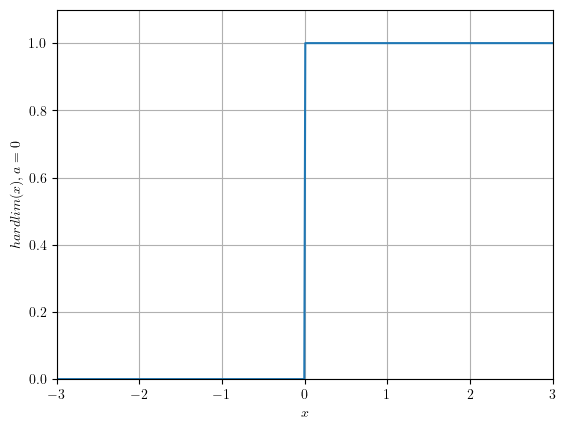
\includegraphics[width=0.5\textwidth]{img/hardlim1.png}
    \caption{The typical hard limit transfer function with fixed $a$, and fixed range for $x$ in $[0,1]$.}
\end{figure}
If we allow modification of the inhibitory value, that is, the zero, by putting it to another variable $a$, the function turns into the dynamic hard limit function, 
\begin{equation}
    \texttt{varhardlim}[x] = \begin{cases}
        0 & x < a\\
        1 & x \geq a
    \end{cases}
\end{equation}
Actually, you can even give the function the value range of absolute jump to be more than $[0,1]$, though fundamentally, according to the logical design, it is not interpretable to anything substantial. 
\begin{figure}[h!]
    \centering
    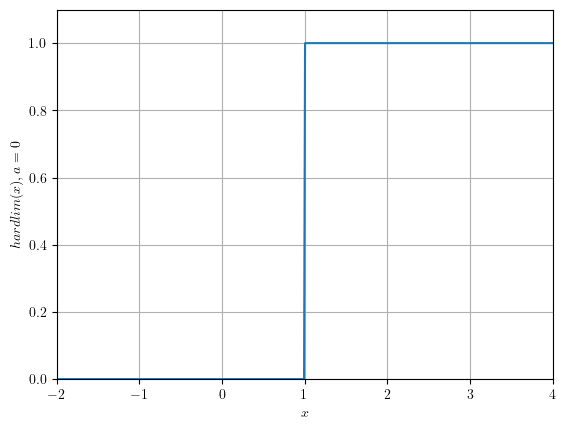
\includegraphics[width=0.5\textwidth]{img/hardlim3.png}
    \caption{The typical hard limit transfer function with variable inhibition $a$, and fixed range for $x$ in $[0,1]$.}
\end{figure}
\subsection{Symmetric hard limit (\texttt{hardlims[x]})}
This one is a variation of \texttt{hardlim}, in which the discrete binary channel is $\{-1,+1\}$ instead. Hard limit is more fitting for probability of logic setting, while symmetric hard limit is more favourable in certain specification, for example, for fuzzy logical domain or directed value functions. Coincidentally, this is also the range that certain sigmoidal variation takes place. Symmetric hard limit is then defined by
\begin{equation}
    \texttt{hardlims}[x] = \begin{cases}
        -1 & x < 0\\
        +1 & x \geq 0 
    \end{cases}
\end{equation}
\begin{figure}[t!]
    \centering
    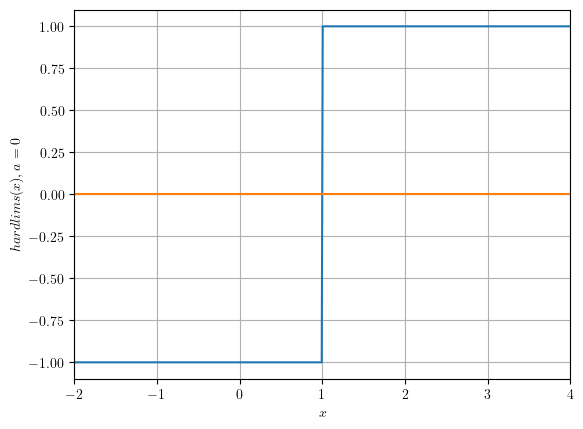
\includegraphics[width=0.5\textwidth]{img/symhardlim.png}
    \caption{The typical symmetric hard limit transfer function with static inhibition $a$, and fixed range for $x$ in $[-1,+1]$. As specified, this is the normal-extended range.}
\end{figure}
\subsection{Linear family (\texttt{satlin[x]}, \texttt{satlins[x]}, \texttt{purelin[x]})}
There are many ways to structure the linear input-output processing node. Usually, we will have the pure linear channel \texttt{purelin}, the saturating linear channel \texttt{satlin}, and the symmetric variation of the saturating linear channel \texttt{satlins}. Because they belong to the same family. The linear one is simple.
\begin{equation}
    \texttt{purelim}[x] = x
\end{equation}
For saturating linear, we have its signal inhibited toward the two ends: 
\begin{equation}
    \texttt{satlin}[x] = \begin{cases}
        0 & x < 0\\
        x & 0 \leq x \leq 1\\
        1 & x > 1
    \end{cases}
\end{equation}
A generalization of this is taken in the form of a functional $f(x)$ enclosed within this range. That is, 
\begin{equation}
    \texttt{varsatlin}[x] = \begin{cases}
        0 & x < 0\\
        f(x) & 0 \leq x \leq 1\\
        1 & x > 1
    \end{cases}
\end{equation}
which might lead to undesired behaviours or simply non-continuous values, but we will have to resolve that later on. If ever. And finally, the symmetric version of the saturating linear functional, 
\begin{equation}
    \texttt{satlin}[x] = \begin{cases}
        -1 & x < 0\\
        x & 0 \leq x \leq 1\\
        1 & x > 1
    \end{cases}
\end{equation}
which will also have the same generalized form. 
\begin{figure}[h!]
    \centering
    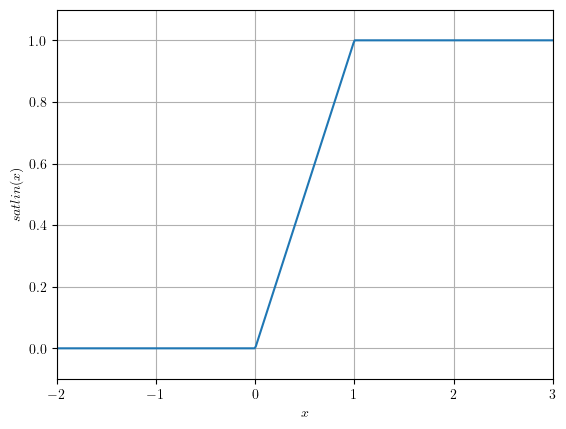
\includegraphics[width=0.5\textwidth]{img/saturatinglin.png}
    \caption{The saturating linear with linear region of $[0,1]$. A smoother variation would be something like sigmoidal functions, that is.}
\end{figure}
\begin{figure}[h!]
    \centering
    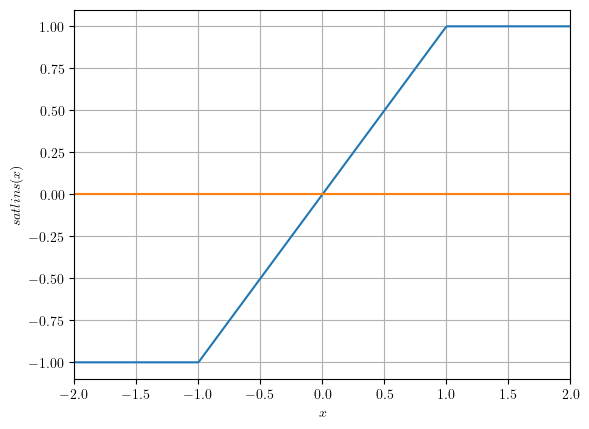
\includegraphics[width=0.5\textwidth]{img/symsatlins.png}
    \caption{The symmetric saturating linear with linear region of $[-1,1]$, a positive-negative variation of the saturating linear.}
\end{figure}
\subsection{Sigmoid (\texttt{sigmoid[x]}) and log-sigmoid (\texttt{logsigmoid[x]})}
The sigmoid function is fairly simple. Instead of giving piecewise saturating condition, we find the expression that gives pairwise, two-sided continuously saturated function, expressed by: 
\begin{equation}
    \texttt{sigmoid}[x] = \frac{1}{1+ e^{-x}}
\end{equation}
\begin{figure}[h!]
    \centering
    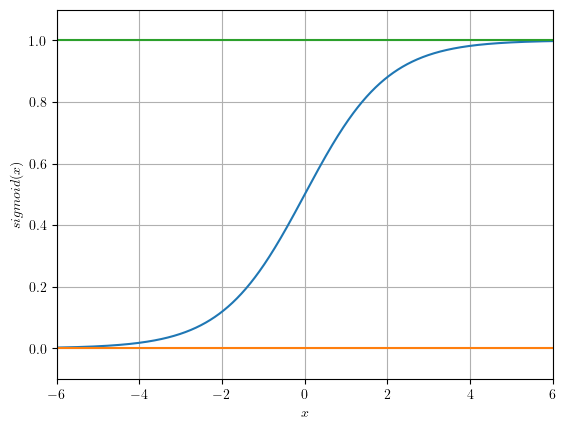
\includegraphics[width=0.5\textwidth]{img/sigmoid.png}
    \caption{The sigmoidal function channel}
\end{figure}
A fairly complicated and often reductive version of it is the log-sigmoid function, as
\begin{equation}
    \texttt{logsigmoid}[x] = \log{\left(\frac{1}{1+ e^{-x}}\right)} = -\log{(1+ \exp{(-x)})}
\end{equation}
Interestingly, the differentiation operator on log-sigmoid gives the sigmoid function, while sigmoid's differentiation gives $\texttt{sigmoid}[x](1-\texttt{sigmoid}[x])$. 
\begin{figure}[h!]
    \centering
    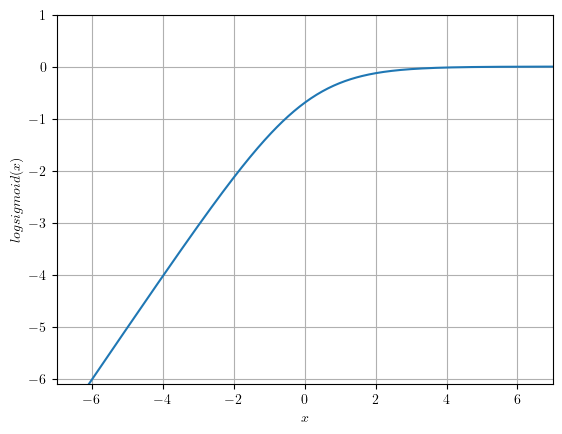
\includegraphics[width=0.5\textwidth]{img/logsigmoid.png}
    \caption{The logarithmic sigmoidal function channel. Notice that the range of \texttt{logsigmoid} is $[-\infty, 0]$, making it somewhat weird of a choice for a transfer function.}
\end{figure}
\subsection{Hyperbolic tangent (\texttt{tansig[x]})}
The hyperbolic tangent the adoption of the hyperbolic function to be transfer function. As such, its range also lies in $[-1,1]$, making it on par with variations of symmetric saturation function. Normally, we would regard this as the somewhat narrow (by width) symmetric version of sigmoid. It is formulated as: 
\begin{equation}
    \texttt{tansig}[x] = \frac{\exp{(x)} - \exp{(-x)}}{\exp{(x)} + \exp{(x)}}
\end{equation}
Also interestingly, hyperbolic tangent is self-referential, evidentual of the derivative:
\begin{equation*}
    \frac{d}{dx} \tanh{(x)} = 1 - \tanh^{2}{(x)}
\end{equation*}
\begin{figure}[H]
    \centering
    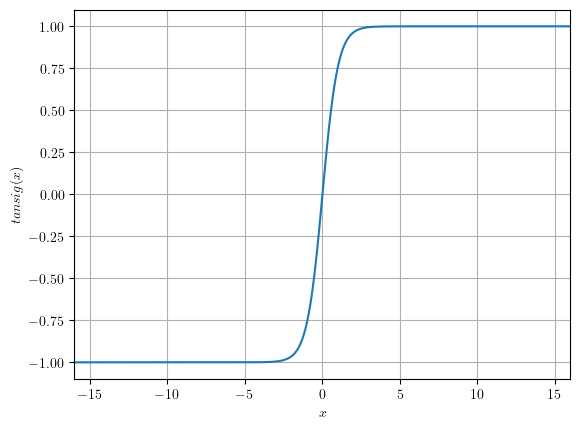
\includegraphics[width=0.5\textwidth]{img/tansig.png}
    \caption{The hyperbolic tangent transfer function channel.}
\end{figure}
The uses of those function can be interpreted to be quite similar to how we can formulate the binary classification, or binary categorization problem-solving solution. 

\section{Deep learning-theoretic activation functions}

The modern landscape provides us the need of variations of activation functions, for multitude of approach and complex models construction. As such, there might be more than forty activation functions being used as design principle throughout the field, belong to certain families, and of certain behavioural classes. Based on reports (\cite{dubey2022activationfunctionsdeeplearning}), in this section, we would like to recite those activation functions and their analysis of usage. 

\subsection{Logistic Sigmoid and Tanh-based}
The first class of activation function is the \textit{logistic, hyperbolic tangent-based} activation functions used in the varied traditional setting. The pitfall of themselves however, is the fact that they are a kind of \textit{bounded activation}, usually in range $[0,1]$ of arbitrary low-end region. While being finite bound, smooth convergence on either side of negative and positive creates the problem of \textit{saturating dilemma} - where output is entirely diminished on either end because of the natural gradient-based learning template. Attempts that have been made to improve on such problem, gives us this section in particular. 

First, is the \textit{scaled Hyperbolic Tangent}\index{scaled Hyperbolic Tangent}, or \texttt{sTanh}$[x]$, defined by 
\begin{equation}
    \texttt{sTanh}[x] = A\times \texttt{Tanh}(B\times x)
\end{equation}
with the output range in $[-A,A]$. A \textit{parametric sigmoid function} (PSF) can also be defined, bounded function represented by 
\begin{equation}
    \texttt{PSF}[x] = \frac{1}{(1+\exp{(-1)})^{m}}
\end{equation}
where $m$ is a hyperparameter. The gradient flow is improved for higher value of $m$, however, there is not so much report about why this is the case, and what would happen for a large network or large complex structure to utilize large $m$. In similar fashion, the \textit{Rectified Hyperbolic Secant} (\texttt{Resech}$[x]$) is differentiable, symmetric, which is given as: 
\begin{equation}
    \texttt{ReSech}[x] = x\times \texttt{Sech}[x]
\end{equation}
with the normalized output range of $[-1,1]$, and is also still susceptible to vanishing gradient for both large positive and large negative inputs. The training of deep network, as we suspected of their usage, become difficult due to the uniform slope of the logistic sigmoid and tangent activation function near the origin. While a solution is not possible, a scaled version of such activation, Scaled Sigmoid or \texttt{sSigmoid} can be created, defined as 
\begin{equation}
    \texttt{sSigmoid}[x] = (4\times \texttt{Sigmoid}[x]-2)
\end{equation}
with output range in $[-2,2]$ and the Penalized Tanh (\texttt{pTanh}), defined by 
\begin{equation}
    \texttt{pTanh}[x] = \begin{cases}
        \texttt{Tanh}[x] & x \geq 0 \\
        a\texttt{Tanh}[x] & x < 0
    \end{cases}
\end{equation}
with the output range in $[-a,1]$ where $a\in(0,1)$ (why the heck?). Nevertheless, the effect of vanishing gradient is well, still an empirical problem to take care of even with such engineering. 

An attempt to overcome vanishing gradient is by defining and using a \textit{noisy activation function}. This is by controlling or adding the noisy gradient landscape, that allow activation function to pick up momentum in smooth regions. Well, we have a few one, includes \textit{Hexpo function}, 
\begin{equation}
    \texttt{Hexpo}[x] = 
    \begin{cases}
        -a \times (\exp{-x/b}-1) & x \geq 0 \\
        c\times (\exp{x/d}-1) & x < 0
    \end{cases}    
\end{equation}
in the output range of $[-c,a]$. The next one, well, is the sigmoid-weighted linear unit, \texttt{SiLU} function, of 
\begin{equation}
    \texttt{SiLU}[x] = x\times \texttt{Sigmoid}[x]
\end{equation}
in the output range of $(-0.5,\infty)$. An improved logistic sigmoid, \texttt{ISigmoid} is also developed by using piecewise combination of sigmoidal and linear functions, 
\begin{equation}
    \texttt{ISigmoid}[x] = \begin{cases}
        \alpha\times (x-a) + \texttt{Sigmoid}[a] & x \geq a \\
        \texttt{Sigmoid}[x] & -a<x < a\\
        \alpha\times (x-a) + \texttt{Sigmoid}[a] & x \geq -a
    \end{cases}
\end{equation}
in the output range of $(-\infty, \infty)$ - which is quite big, however, without knowing much about the shape and total asymptotic analysis, we cannot know for sure what happens. The Elliott function and Soft-Root-Sign (SRS) functions are also, well, designed of the same goal, 
\begin{equation}
    \texttt{Elliott}[x] = \frac{x}{2(1+|x|)}+\frac{1}{2} , \quad \texttt{SRS}[x] = \frac{x}{(x/\alpha)+\exp{(-x/\beta)}}
\end{equation}
for output range $[0,1]$ and $[(\alpha\times\beta)/(\beta-\alpha\times e),\alpha]$, for the \texttt{SRS} can vary within two parameters configuration. Nevertheless, the issue of vanishing gradient still persists. 
\subsection{Rectified Activation Functions}
Rectified activation function belongs to a class of functions called the \textit{ramp functions}. Per definition, a ramp function is a unary real function, whose graph usually can be segmented into two sections. The most famous example, of course, is the Heaviside step function multiplied by a linear function, 
\begin{equation}
    R(x) = xH(x) = \begin{cases}
        x & x \geq 0 \\
        0 & x < 0
    \end{cases}
\end{equation}
or the mean of an independent variable and its absolute value, 
\begin{equation}
    R(x) = \frac{x+|x|}{2}
\end{equation}
or, again, of the Heaviside integral, 
\begin{equation}
    R(x):= \int^{\pi}_{-\infty}H(\xi)\:d\xi
\end{equation}
or a tad bit crazier but feels more at home, the limit functional class, for example, 
\begin{equation}
    R(x) := \lim_{a\to\infty} \begin{cases}
        1/a & x = 0 \\
        x/(1-\exp{(-ax)}) & x \neq 0 
    \end{cases}
\end{equation}
In a sense, the definition of a step function can be also considered similar to the ramp function. However, usually, ramp function requires its domain to be continuous, while step function usually is not. The Heaviside step function with linear multiplier above, is also coincidentally, the expression for the \textit{standard rectified activation function}, \texttt{ReLU}, which is indeed just defined as
\begin{equation}
    \texttt{ReLU}[x] = max(0,x) = \begin{cases}
        x & x \geq 0 \\
        0 & x < 0
    \end{cases}
\end{equation}
The range of nonzero operational value is then $[0,\infty)$, as accordance. Funnily enough, if we are to use \texttt{ReLU}, we are actually switching the vanishing gradient problem from one to another, which is now into the problem of vanishing gradient in the negative region. Nevertheless, it does not stop the dumb fuck from using it, so it is good anyway. 

What is the usage of this kind of function, especially \texttt{ReLU}, you ask? Unrelated to machine learning and stuff, then, quite a lot. At least in terms of rectified function, \texttt{ReLU} takes the analogy to \textit{half-wave rectification} in AC circuit (basically an AC-DC conversion circuit with rectified output, that certainly improves on the unfortunate reality that AC circuit, if taken as DC on a straight wiring, will have loops or missing reverse current flow). Hence, you would see this type of function in a lot of digital signal processing from the onset than not, before even machine learning or statistical regression is even a thing. In fact, Macaulay's bracket was developed to denote the ramp function to solve the \textit{Euler-Bernoulli beam} problem for elasticity of beams. Ramp function in domain transformation, is the positive part of any given real function $f(x)$. Hence, we would often see \texttt{ReLU} and the like be described as $\mathbb{R}\to\mathbb{R}_{0}^{+}$, though this convention will be kind of broken in certain cases. In finance, they are used for shit like call options. And finally for us, we use it in the activation function of deep neural network units. 

\subsubsection{Properties}

For ramp functions and the like, the following often holds. 
\begin{definition}[Properties]
    For a standard ramp function that \texttt{ReLU} is in, it is defined as: 
    \begin{equation}
        R(x)=xH(x) = \int^{\pi}_{-\infty} H(x') \: dx' = \int_{-\infty}^{\infty} H(x')H(x-x')\:dx'=H(x) * H(x)
    \end{equation}
    Where $H(x)$ is the Heaviside step function, and $*$ denotes convolution. The derivative is then $R'(x)=H(x)$ of the integrable Heaviside. 
\end{definition}

The ramp function also have the simple result of being non-negative in the domain (which is usually explained pretty nice). 
\begin{proposition}
    In the domain of $R(x)$ for all $x\in D \subset \mathbb{R}$, the ramp function is non-negative, i.e. $R\geq 0$, and $|R(x)=R(x)|$. 
\end{proposition}
\begin{definition}
    The second derivative of ramp function satisfies the differential equation 
    \begin{equation}
        \frac{d^{2}}{dx^{2}} R(x-x_0) = \delta(x-x_0)
    \end{equation}
    for $\delta(x)$ the Dirac delta. 
\end{definition}
Finally, we have the property of \textit{iteration invariance} for a series of ReLU form. 
\begin{theorem}
    For all $x\in D\subset \mathbb{R}$, we have 
    \begin{equation}
        R(R(x)) = R(x)
    \end{equation}
\end{theorem}
\begin{proof}
    We have 
    \begin{equation}
        R(R(x)) := \frac{R(x)+|R(x|}{2} = \frac{R(x)+R(x)}{2} = R(x)
    \end{equation}
    by the non-negativity property. 
\end{proof}
\subsubsection{Variation 1 - Non-negativity}
